\documentclass[12pt]{article}

\usepackage{sbc-template}
\usepackage{graphicx,url}
%\usepackage[brazil]{babel}   
\usepackage[utf8]{inputenc}  
\usepackage{amsmath}
\usepackage{float}
     
\sloppy

\title{TP02 - Problema dos k-Centros}

\author{Diego H. Xavier dos Santos\inst{1}, Marcos V. Nunes Reis\inst{1}, Vitor Daniel Silva Melo\inst{1}}


\address{Instituto de Ciências Exatas e Informática -- Pontifícia Universidade\\ Católica de Minas Gerais
  (PUC-MG)\\
  Caixa Postal 1.162 -- 30.140-108 -- Belo Horizonte -- MG -- Brazil
  \email{dhxsantos@sga.pucminas.br, marcos.reis.1537860@sga.pucminas.br,}\email{vdsmelo@sga.pucminas.br}
}

\begin{document} 

\maketitle
     
\begin{resumo}
O problema dos $k$-centros consiste em selecionar um conjunto de até $k$ vértices de um grafo de forma a minimizar a maior distância entre qualquer vértice e o centro mais próximo. Esse problema possui diversas aplicações em agrupamento de dados, localização de instalações e planejamento logístico, sendo conhecido por sua elevada complexidade computacional. Neste trabalho foram implementadas e comparadas duas abordagens para sua resolução: uma solução exata baseada em Branch and Bound e uma solução aproximada baseada na heurística \textit{farthest-first} proposta por Gonzalez. Os algoritmos foram avaliados utilizando as quarenta instâncias de p-medianas disponibilizadas pela OR-Library. Os resultados mostram que a heurística de Gonzalez produz soluções de boa qualidade em tempos muito reduzidos, enquanto a abordagem exata encontra dificuldades para resolver instâncias maiores devido ao crescimento combinatorial do espaço de busca\cite{cormen2009,dasgupta2006}. A comparação evidencia o compromisso entre qualidade da solução e tempo de execução característico de problemas NP-difíceis.
\end{resumo}

\section{Introdução}

Problemas de agrupamento e localização estão presentes em diversas áreas da computação, pesquisa operacional e ciência de dados. Em aplicações como posicionamento de centros de distribuição, instalação de serviços públicos, projeto de redes de comunicação e agrupamento de elementos semelhantes, frequentemente deseja-se selecionar um conjunto reduzido de representantes capazes de atender adequadamente todos os elementos de interesse.

Nesse contexto, o problema dos $k$-centros busca determinar um conjunto de até $k$ vértices de um grafo, denominados centros, de forma a minimizar a pior distância entre qualquer vértice e seu centro mais próximo. Diferentemente do problema das p-medianas, que minimiza a soma das distâncias, o problema dos $k$-centros preocupa-se especificamente com o pior caso, tornando-se particularmente adequado para aplicações nas quais se deseja garantir um limite máximo de atendimento.

O problema é conhecido por ser NP-difícil\cite{cormen2009,dasgupta2006}, o que torna inviável a obtenção de soluções ótimas para instâncias de grande porte por meio de métodos exatos. Em razão disso, a literatura apresenta diversas abordagens aproximadas capazes de produzir soluções de boa qualidade em tempo polinomial. Entre elas, destaca-se o algoritmo proposto por Gonzalez, que possui garantia teórica de aproximação igual a 2\cite{gonzalez1985,hochbaum1985}.

O objetivo deste trabalho é implementar e comparar duas estratégias para a resolução do problema dos $k$-centros: uma abordagem exata baseada em Branch and Bound e uma abordagem aproximada baseada na heurística de Gonzalez. Os algoritmos são avaliados utilizando as quarenta instâncias da OR-Library\cite{beasley1990} originalmente propostas para o problema das p-medianas, permitindo analisar tanto a qualidade das soluções obtidas quanto o comportamento computacional de cada método à medida que o tamanho das instâncias aumenta.

\section{Fundamentos Teóricos}

\subsection{Problema dos \textit{k}-Centros}

Considere um grafo ponderado $G=(V,E)$ e um inteiro positivo $k$. O problema dos $k$-centros consiste em selecionar um conjunto de vértices $C \subseteq V$, com $|C| \leq k$, de modo a minimizar o raio da solução.

Formalmente, o raio associado a um conjunto de centros $C$ é definido por

\[
R(C)=\max_{v \in V}\min_{c \in C} d(v,c),
\]

onde $d(v,c)$ representa a distância de menor caminho entre os vértices $v$ e $c$.

A expressão interna determina a distância entre um vértice e seu centro mais próximo, enquanto a maximização externa identifica o vértice pior atendido pela solução. Dessa forma, o objetivo do problema é minimizar a maior distância existente entre qualquer vértice do grafo e o centro mais próximo.

O problema possui aplicações em localização de instalações, posicionamento de servidores, planejamento logístico e agrupamento de dados, sendo frequentemente utilizado quando o critério de qualidade está associado ao pior caso de atendimento.

\subsection{Complexidade Computacional}

O problema dos $k$-centros pertence à classe dos problemas NP-difíceis. Consequentemente, não são conhecidos algoritmos de tempo polinomial capazes de encontrar soluções ótimas para instâncias arbitrárias.

Uma abordagem exaustiva consistiria em avaliar todos os subconjuntos de vértices com tamanho $k$. O número de combinações possíveis é dado por $\binom{n}{k}$, onde $n=|V|$ representa o número de vértices do grafo. Esse valor cresce rapidamente mesmo para instâncias moderadas, tornando a enumeração completa inviável na prática.

Devido a essa dificuldade computacional, algoritmos aproximados desempenham papel fundamental na resolução de instâncias de maior porte, oferecendo soluções próximas da ótima em tempos significativamente menores.

\subsection{Heurística de Gonzalez}

A solução aproximada implementada baseia-se no algoritmo \textit{farthest-first traversal} proposto por Gonzalez\cite{gonzalez1985}. A ideia central consiste em selecionar iterativamente novos centros nos vértices que se encontram mais distantes dos centros já escolhidos.

Inicialmente, é selecionado um vértice arbitrário como primeiro centro. Na implementação desenvolvida, o vértice de índice zero é utilizado como ponto de partida, tornando a execução determinística e facilitando a reprodução dos experimentos.

Após a escolha de cada centro, é executado o algoritmo de Dijkstra para calcular as distâncias entre esse centro e todos os demais vértices do grafo. Para cada vértice $v$, mantém-se o valor \texttt{menorDist}[v],

que representa a menor distância entre $v$ e qualquer centro já selecionado.

Em seguida, o próximo centro é escolhido como o vértice cujo valor de \texttt{menorDist} é máximo, ou seja, o vértice atualmente pior atendido pela solução parcial. Após a inclusão do novo centro, as distâncias mínimas são atualizadas e o processo é repetido até que $k$ centros tenham sido selecionados.

Ao final da execução, o raio da solução é obtido pela expressão 

\[
R(C)=\max_{v \in V} \texttt{menorDist}[v].
\]

A implementação também disponibiliza um método auxiliar para recalcular o raio de um conjunto arbitrário de centros, utilizado durante os testes de validação.

Como o algoritmo executa uma chamada ao Dijkstra para cada centro selecionado, sua complexidade temporal é dada por $O(k \cdot m \log n)$, onde $n$ representa o número de vértices e $m$ o número de arestas do grafo. O consumo de memória é da ordem de $O(n+m)$.

Além de sua eficiência prática, o algoritmo de Gonzalez possui garantia teórica de aproximação igual a $2$, assegurando que o raio obtido nunca excede o dobro do raio ótimo.

\subsection{Solução Exata}

A abordagem exata implementada realiza uma busca sistemática por todos os subconjuntos de vértices com cardinalidade igual a $k$. Cada subconjunto representa uma possível escolha de centros para o problema.

A busca é conduzida por meio de uma estratégia recursiva de retrocesso (\textit{backtracking}). Em cada nível da árvore de busca é escolhido um novo vértice para compor a solução parcial. Quando são selecionados exatamente $k$ centros, obtém-se uma solução completa e seu raio é calculado.

Para acelerar a avaliação das soluções, utiliza-se previamente uma matriz de distâncias entre todos os pares de vértices. Durante a construção de uma solução parcial, mantém-se um vetor denominado \texttt{menorDist}, no qual cada posição armazena a distância do vértice correspondente ao centro mais próximo já escolhido.

Sempre que um novo centro é adicionado à solução parcial, o vetor é atualizado segundo $\texttt{menorDist\_[v]} = \min(\texttt{menorDist\_[v]}, d(c,v))$, onde $c$ representa o centro recém-adicionado.

Quando uma solução completa é encontrada, o raio correspondente é determinado pelo maior valor presente em \texttt{menorDist}. Caso esse raio seja inferior ao melhor resultado conhecido até então, a solução passa a ser armazenada como a melhor solução encontrada.

A implementação emprega uma poda estrutural simples. Considere uma chamada recursiva na qual ainda faltam selecionar $r$ centros e existem apenas $a$ vértices candidatos disponíveis. Se $a < r$, torna-se impossível completar uma solução válida e o ramo correspondente é imediatamente descartado.

Além disso, o algoritmo utiliza como cota superior inicial o resultado produzido pela heurística de Gonzalez. Dessa forma, qualquer solução completa encontrada somente é armazenada caso apresente raio inferior ao obtido pela heurística.

Um aspecto importante é que não foi utilizada poda baseada no raio parcial da solução. Isso ocorre porque a inclusão de novos centros pode apenas reduzir as distâncias mínimas dos vértices, fazendo com que o raio seja monotonicamente não crescente ao longo da construção da solução. Consequentemente, um raio parcial elevado não implica necessariamente que o raio final também será elevado.

Como o número de combinações possíveis cresce segundo $\binom{n}{k}$, o tempo de execução torna-se rapidamente proibitivo para instâncias maiores. Por essa razão, foi incorporado um mecanismo de interrupção por tempo limite (\textit{timeout}), configurado em segundos. Caso esse limite seja atingido, a busca é encerrada e o melhor resultado encontrado até o momento é retornado, sem garantia de otimalidade.

Embora a abordagem seja capaz de encontrar soluções ótimas para instâncias pequenas, o crescimento combinatorial do espaço de busca restringe sua aplicabilidade prática em instâncias de maior porte, reforçando a importância de métodos aproximados para o problema dos $k$-centros.

\section{Implementação}

Esta seção descreve os principais aspectos da implementação desenvolvida para a resolução do problema dos $k$-centros. O projeto foi implementado integralmente em Java e organizado em módulos independentes para leitura das instâncias, representação dos grafos, cálculo de menores caminhos e execução dos algoritmos de solução.

\subsection{Organização do Projeto}

A implementação foi dividida em classes especializadas, cada uma responsável por uma etapa específica do processamento. A Tabela~\ref{tab:arquivos} apresenta um resumo dos principais arquivos do projeto.

\begin{table}[h] 
\centering 
\caption{Principais componentes da implementação} \label{tab:arquivos} 
\begin{tabular}{ll} 
\hline 
\textbf{Arquivo} & \textbf{Função} \\ 
\hline 
Grafo.java & Representação do grafo em CSR \\ 
LeitorPmed.java & Leitura das instâncias da OR-Library \\ 
Dijkstra.java & Cálculo de menores caminhos \\ 
Distancias.java & Matriz de distâncias entre todos os pares \\ 
Gonzalez.java & Heurística aproximada \\ 
Exata.java & Busca exata com timeout \\ 
Raio.java & Avaliação e validação de soluções \\ 
Principal.java & Execução dos experimentos \\ 
Testes.java & Casos de teste automatizados \\ 
\hline 
\end{tabular} 
\end{table}

Essa divisão permitiu desacoplar os diferentes componentes do sistema, facilitando tanto os testes quanto a reutilização de código entre os algoritmos implementados.

\subsection{Leitura das Instâncias da OR-Library}

As instâncias utilizadas são provenientes da OR-Library e seguem o formato tradicional do problema das p-medianas. A primeira linha de cada arquivo contém o número de vértices $n$, o número de arestas $m$ e o valor do parâmetro $k$.

As linhas seguintes descrevem as arestas do grafo no formato $u \quad v \quad custo$,

onde os vértices são indexados a partir de 1 e os custos representam pesos não negativos.

Para minimizar o tempo de leitura, foi implementado um leitor próprio baseado em \texttt{BufferedInputStream}, evitando o uso da classe \texttt{Scanner}, que apresenta desempenho inferior em arquivos de grande porte.

\subsection{Tratamento de Arestas Paralelas}

Durante a análise das instâncias observou-se a presença de arestas paralelas entre alguns pares de vértices. Conforme especificado pela documentação da OR-Library, quando múltiplas arestas conectam o mesmo par de vértices, deve ser considerado o custo da última ocorrência no arquivo.

Para implementar essa regra, utilizou-se uma estrutura baseada em \texttt{HashMap}. Cada par de vértices é associado a uma chave única, permitindo que leituras posteriores sobrescrevam automaticamente valores anteriores.

Esse tratamento mostrou-se essencial para reproduzir corretamente os valores ótimos divulgados para as instâncias de referência.

\subsection{Representação do Grafo}

Os grafos foram armazenados utilizando a estrutura \textit{Compressed Sparse Row} (CSR). Nessa representação, todas as arestas são armazenadas em vetores contíguos de memória, reduzindo a quantidade de objetos alocados e melhorando a localidade de cache.

A estrutura é composta por três vetores principais:

\begin{itemize}
\item \texttt{inicio}: indica onde começa a lista de vizinhos de cada vértice;
\item \texttt{destino}: armazena os vértices adjacentes;
\item \texttt{peso}: armazena os custos das arestas.
\end{itemize}

Para percorrer os vizinhos de um vértice $v$, basta iterar pelos índices compreendidos entre \texttt{inicio[v]} e \texttt{inicio[v+1]-1}.

Essa abordagem apresenta desempenho superior ao uso de listas de adjacência baseadas em objetos, especialmente nas repetidas execuções do algoritmo de Dijkstra.

\subsection{Cálculo das Distâncias}

Tanto a heurística de Gonzalez quanto a solução exata dependem do cálculo de menores caminhos.

Para isso foi implementado o algoritmo de Dijkstra utilizando fila de prioridade baseada em heap binário. A heurística executa o algoritmo a partir de cada novo centro selecionado, enquanto a solução exata utiliza uma matriz de distâncias previamente calculada entre todos os pares de vértices.

A matriz é construída por meio de $n$ execuções independentes do algoritmo de Dijkstra, uma para cada vértice do grafo.

\subsection{Estruturas de Dados e Otimizações}

Algumas otimizações foram incorporadas visando reduzir o tempo de execução dos experimentos.

A fila de prioridade utilizada pelo algoritmo de Dijkstra foi implementada manualmente, evitando o custo associado às estruturas genéricas da biblioteca padrão. Cada elemento da fila é armazenado em um único valor do tipo \texttt{long}, contendo simultaneamente a distância e o identificador do vértice.

Além disso, os vetores auxiliares utilizados pelos algoritmos são reutilizados sempre que possível, reduzindo a quantidade de alocações de memória durante a execução.

Essas otimizações mostraram-se importantes principalmente para as maiores instâncias avaliadas, que possuem até 900 vértices e aproximadamente 16 mil arestas.

\section{Experimentos}

\subsection{Configuração}

Os experimentos foram executados em um ambiente Ubuntu executado sobre o Windows Subsystem for Linux 2 (WSL2). A configuração utilizada foi:

\begin{itemize}
    \item \textbf{Processador:} AMD Ryzen 7 5700U with Radeon Graphics;
    \item \textbf{Memória RAM:} 4,7 GiB;
    \item \textbf{Sistema operacional:} Ubuntu (WSL2), kernel Linux 6.18.33.1-1;
    \item \textbf{Java:} OpenJDK/Java SE 24.0.2 (Java HotSpot 64-Bit Server VM).
\end{itemize}

\subsection{Instâncias Utilizadas}

Foram utilizadas as 40 instâncias clássicas da biblioteca OR-Library, identificadas de \texttt{pmed01} a \texttt{pmed40}. Essas instâncias possuem tamanhos variando de 100 a 900 vértices e diferentes quantidades de centros a serem selecionados.

\begin{table}[H]
\centering
\caption{Resumo das instâncias utilizadas.}
\begin{tabular}{lccc}
\hline
Grupo de instâncias & Quantidade & Faixa de $n$ & Faixa de $k$ \\
\hline
pmed01--pmed05 & 5 & 100 & 5--33 \\
pmed06--pmed10 & 5 & 200 & 5--67 \\
pmed11--pmed15 & 5 & 300 & 5--100 \\
pmed16--pmed20 & 5 & 400 & 5--133 \\
pmed21--pmed25 & 5 & 500 & 5--167 \\
pmed26--pmed30 & 5 & 600 & 5--200 \\
pmed31--pmed34 & 4 & 700 & 5--140 \\
pmed35--pmed37 & 3 & 800 & 5--80 \\
pmed38--pmed40 & 3 & 900 & 5--90 \\
\hline
Total & 40 & 100--900 & 5--200 \\
\hline
\end{tabular}
\label{tab:instancias}
\end{table}

\subsection{Resultados da Heurística de Gonzalez}

A heurística de Gonzalez foi executada sobre as 40 instâncias da OR-Library. Para cada instância, foi calculada a razão de aproximação

\[
\text{Razão} = \frac{\text{raio obtido pela heurística}}{\text{raio ótimo}}.
\]

A Tabela~\ref{tab:gonzalez} apresenta os resultados obtidos.

\begin{table}[h]
\centering
\caption{Resumo dos resultados da heurística de Gonzalez.}
\begin{tabular}{lccc}
\hline
Métrica & Valor \\
\hline
Melhor razão & 1,2373 \\
Pior razão & 1,7872 \\
Razão média & 1,50 \\
Garantia teórica & 2,00 \\
\hline
\end{tabular}
\label{tab:gonzalez}
\end{table}

Observa-se que todas as soluções encontradas respeitaram o limite teórico de aproximação de fator 2. Além disso, a razão média obtida foi aproximadamente 1,50, indicando que, na prática, a heurística produziu soluções significativamente melhores do que o pior caso garantido pela teoria.

A Figura~\ref{fig:gonzalez} mostra que as razões observadas permaneceram concentradas entre aproximadamente 1,24 e 1,79, sem nenhuma violação da garantia teórica. Os resultados sugerem que a heurística apresenta desempenho consistente em diferentes tamanhos de instância, produzindo soluções de boa qualidade com baixo custo computacional.

\begin{figure}[ht]
\centering
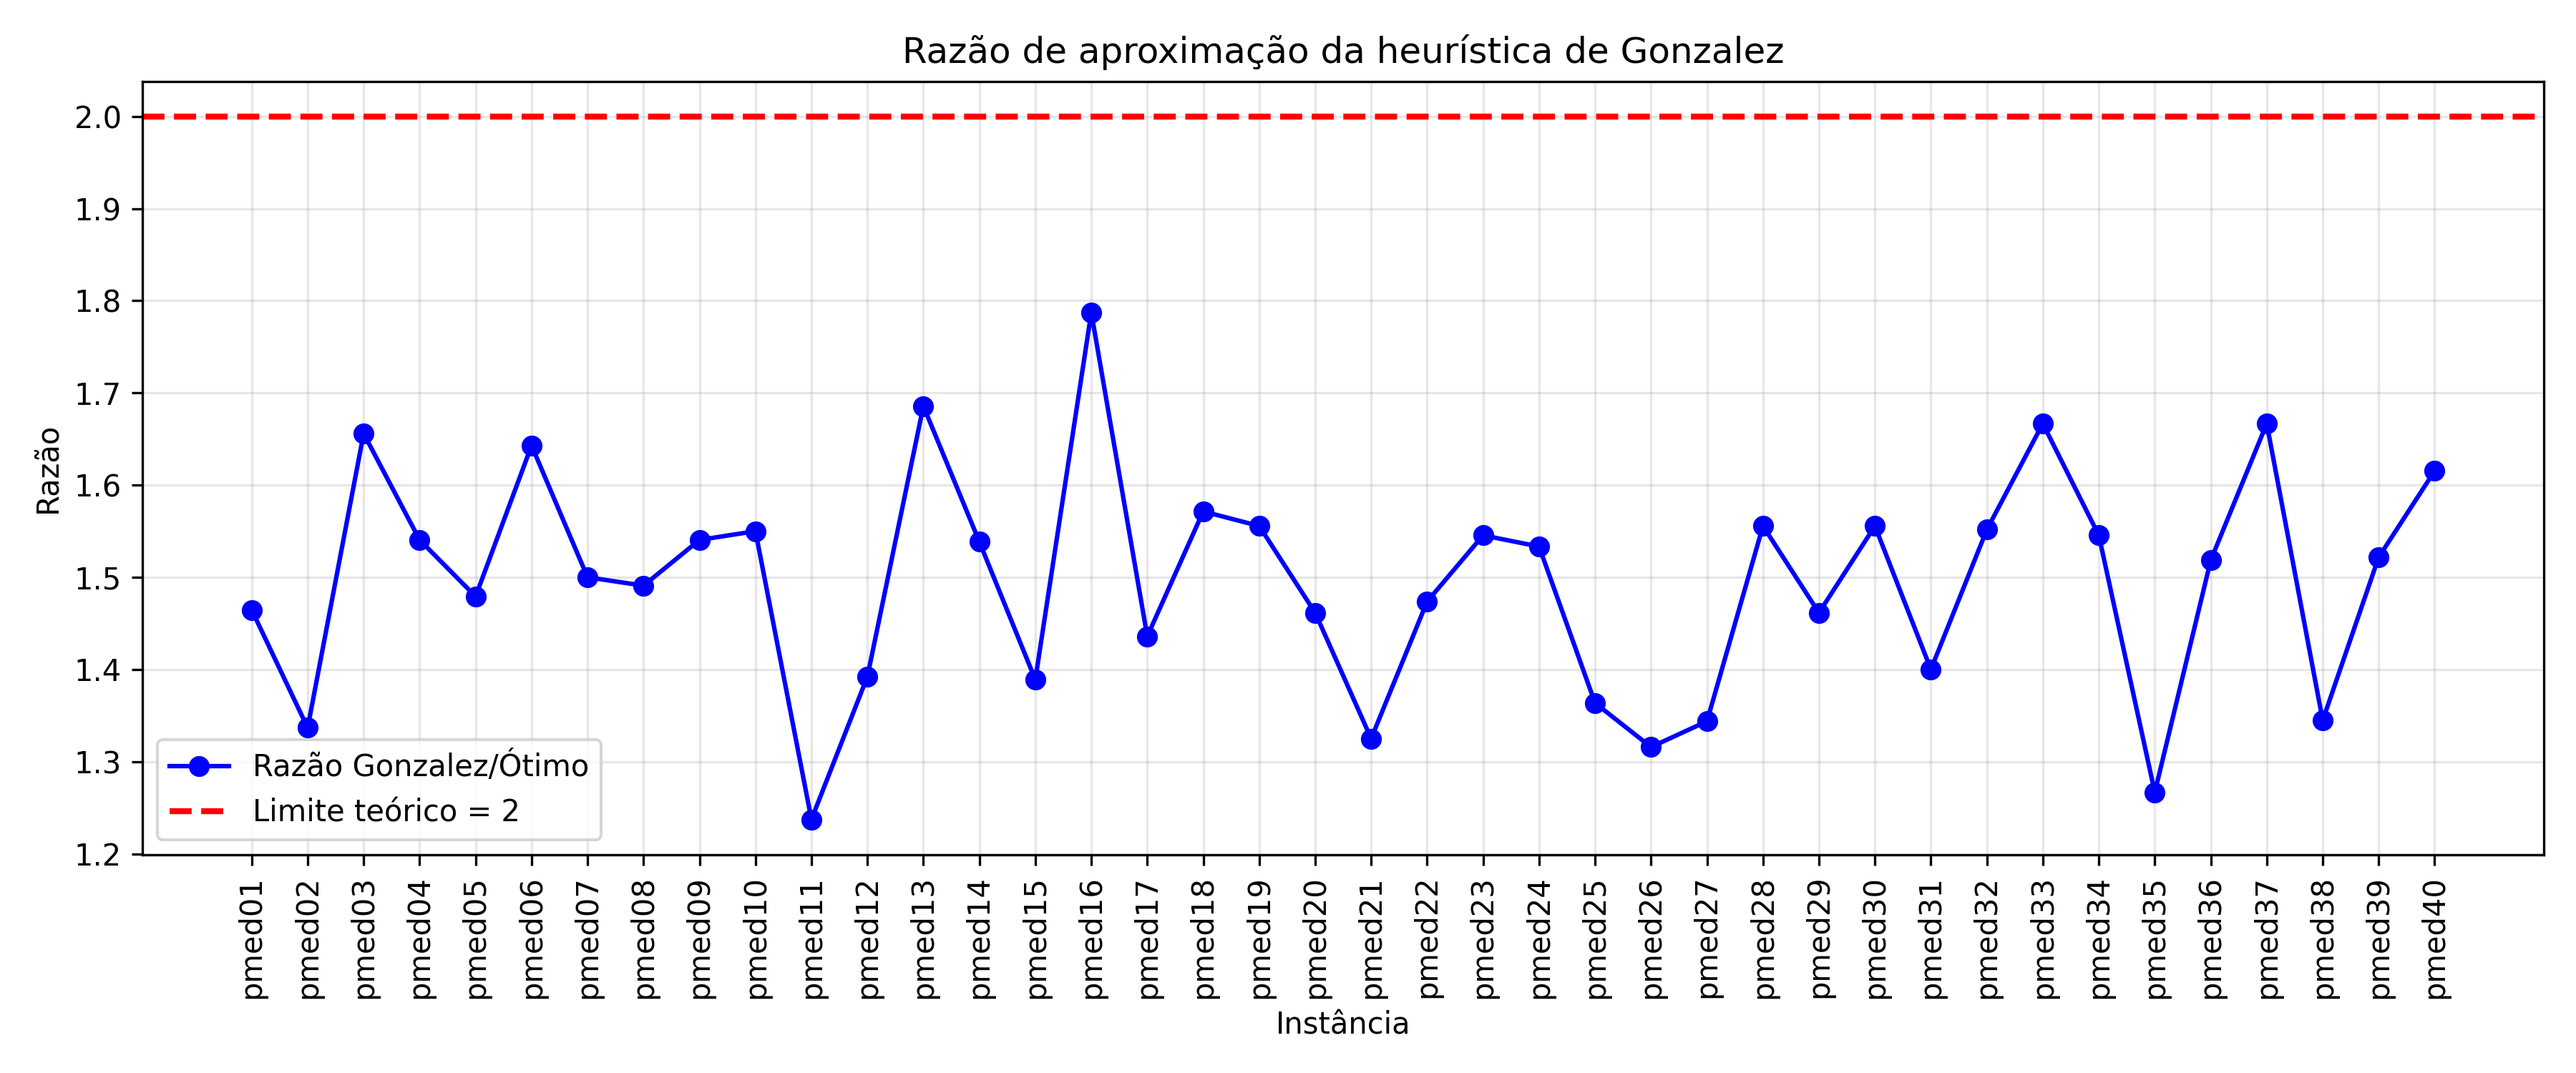
\includegraphics[width=\textwidth]{gonzalez_razao.png}
\caption{Razão de aproximação da heurística de Gonzalez para as instâncias da OR-Library. A linha tracejada indica o limite teórico de aproximação igual a 2.}
\label{fig:gonzalez}
\end{figure}

\subsection{Resultados da Solução Exata}

A solução exata baseada em Branch and Bound foi executada sobre as 40 instâncias da OR-Library, utilizando um limite de tempo de 60 segundos por instância. Os resultados completos encontram-se na Tabela~X.

Dos 40 problemas avaliados, apenas a instância \texttt{pmed01} foi resolvida até a prova de otimalidade, obtendo exatamente o valor ótimo conhecido (127) após aproximadamente 13,6 segundos. Todas as demais instâncias atingiram o limite de tempo estabelecido e foram encerradas com status \texttt{TIMEOUT}.

Apesar disso, o algoritmo foi capaz de encontrar soluções de boa qualidade em diversos casos. O menor gap observado foi de 1,19\% (\texttt{pmed06}), enquanto o maior atingiu 66,67\% (\texttt{pmed33} e \texttt{pmed37}). Em instâncias de menor porte e com valores reduzidos de $k$, os gaps permaneceram relativamente baixos, frequentemente abaixo de 10\%. Entretanto, à medida que o tamanho das instâncias aumentou, a qualidade das melhores soluções encontradas dentro do limite de tempo deteriorou-se gradualmente.

O tempo médio de execução foi próximo de 62 segundos, refletindo o fato de que praticamente todas as execuções consumiram integralmente o orçamento computacional disponível. Além disso, o número de nós explorados na árvore de busca foi elevado. Em algumas instâncias pequenas, como \texttt{pmed02} e \texttt{pmed04}, mais de 20 milhões de nós foram processados antes da interrupção. Mesmo para instâncias maiores, onde as podas reduziram parcialmente a árvore, centenas de milhares de nós ainda precisaram ser avaliados.

Esses resultados evidenciam a dificuldade computacional do problema dos $k$-centros quando tratado por métodos exatos. Embora o algoritmo consiga encontrar soluções viáveis relativamente cedo durante a execução, a comprovação da otimalidade torna-se rapidamente inviável devido ao crescimento combinatório do espaço de busca.

\begin{table}[htbp]
\centering
\caption{Resumo dos resultados da solução exata.}
\begin{tabular}{lc}
\hline
Métrica & Valor \\
\hline
Instâncias avaliadas & 40 \\
Soluções ótimas comprovadas & 1 \\
Timeouts & 39 \\
Menor gap & 1,19\% \\
Maior gap & 66,67\% \\
Tempo médio & 62,6 s \\
Maior número de nós explorados & 43.036.672 \\
\hline
\end{tabular}
\end{table}

Os resultados apresentados na Figura~\ref{fig:gap-exata} mostram a evolução do desvio percentual em relação ao valor ótimo conhecido para cada instância. Observa-se uma grande variação nos gaps, com instâncias pequenas apresentando desvios reduzidos, enquanto instâncias maiores tendem a apresentar degradação significativa da qualidade da solução dentro do limite de tempo estabelecido.

\begin{figure}[htbp]
\centering
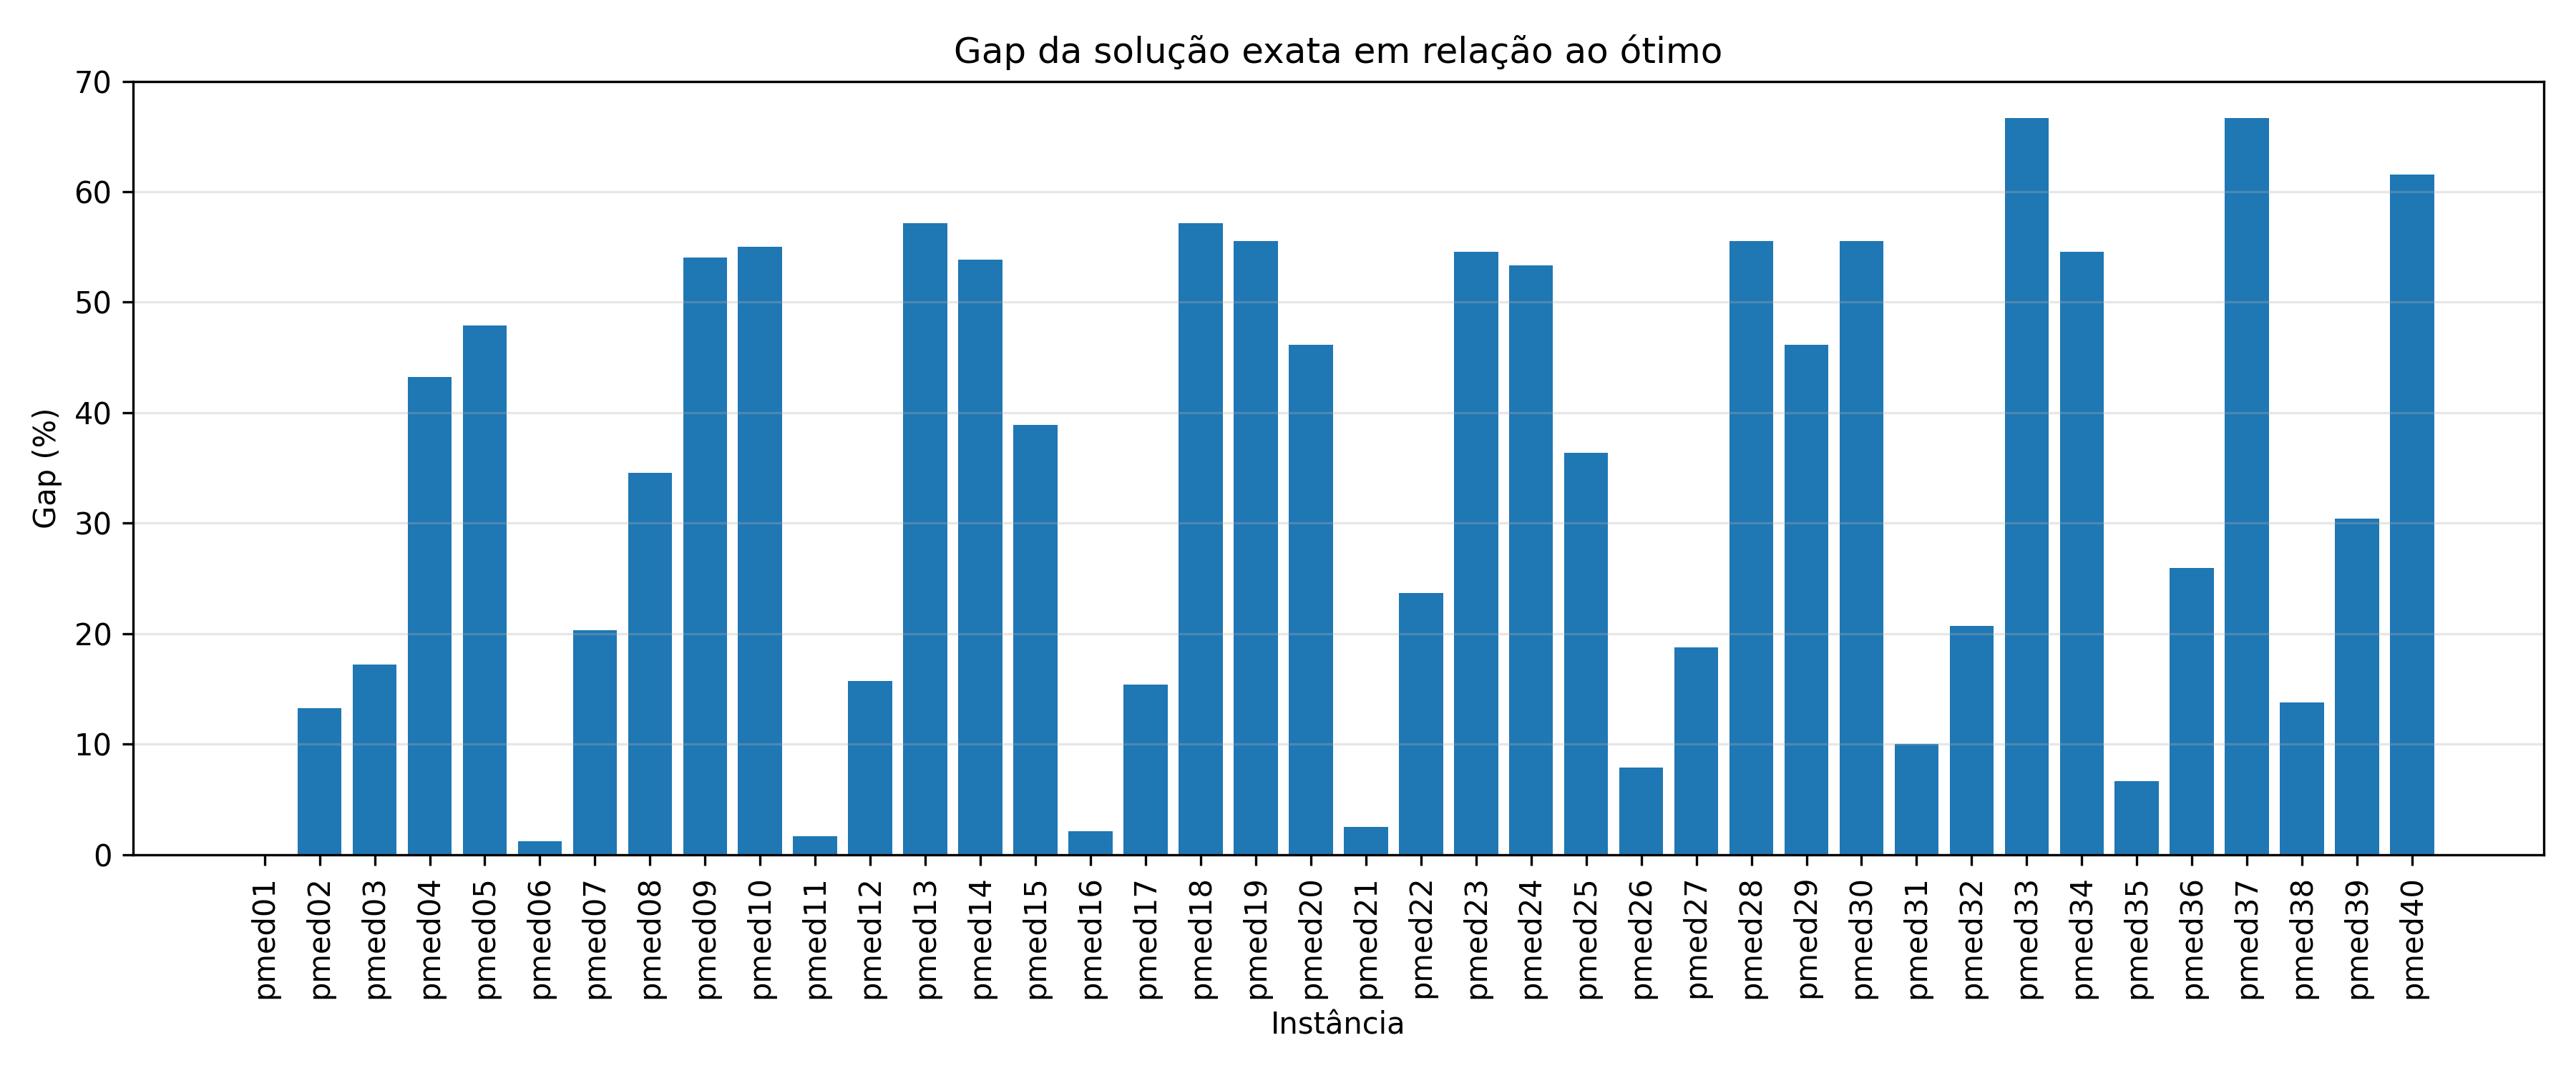
\includegraphics[width=\textwidth]{gap_exata.png}
\caption{Gap percentual da solução exata em relação ao valor ótimo após o limite de tempo de 60 segundos.}
\label{fig:gap-exata}
\end{figure}

\subsection{Comparação entre os Métodos}

A comparação entre a heurística de Gonzalez e a solução exata evidencia o clássico compromisso entre qualidade da solução e tempo de execução.

Em termos de qualidade, a heurística apresentou razão média de aproximação próxima de 1,50, permanecendo sempre abaixo do limite teórico de 2. O melhor resultado observado foi 1,2373 e o pior 1,7872. Esses valores indicam que as soluções produzidas estiveram relativamente próximas do ótimo em todas as instâncias avaliadas.

Por outro lado, a abordagem exata foi capaz de comprovar a otimalidade apenas para a instância \texttt{pmed01}. Nas demais instâncias, o algoritmo atingiu o limite de tempo de 60 segundos sem concluir a exploração completa da árvore de busca.

Em termos de eficiência, a diferença entre os métodos foi ainda mais significativa. A heurística produziu soluções em poucos milissegundos, mesmo para as maiores instâncias, enquanto o Branch and Bound consumiu aproximadamente um minuto por instância e, ainda assim, não conseguiu garantir a otimalidade na maioria dos casos.

Os resultados mostram que a heurística de Gonzalez oferece excelente escalabilidade e produz soluções de boa qualidade em tempo reduzido, enquanto a abordagem exata torna-se rapidamente inviável para instâncias de maior porte devido ao crescimento combinatório do espaço de busca.

\begin{figure}[H]
\centering
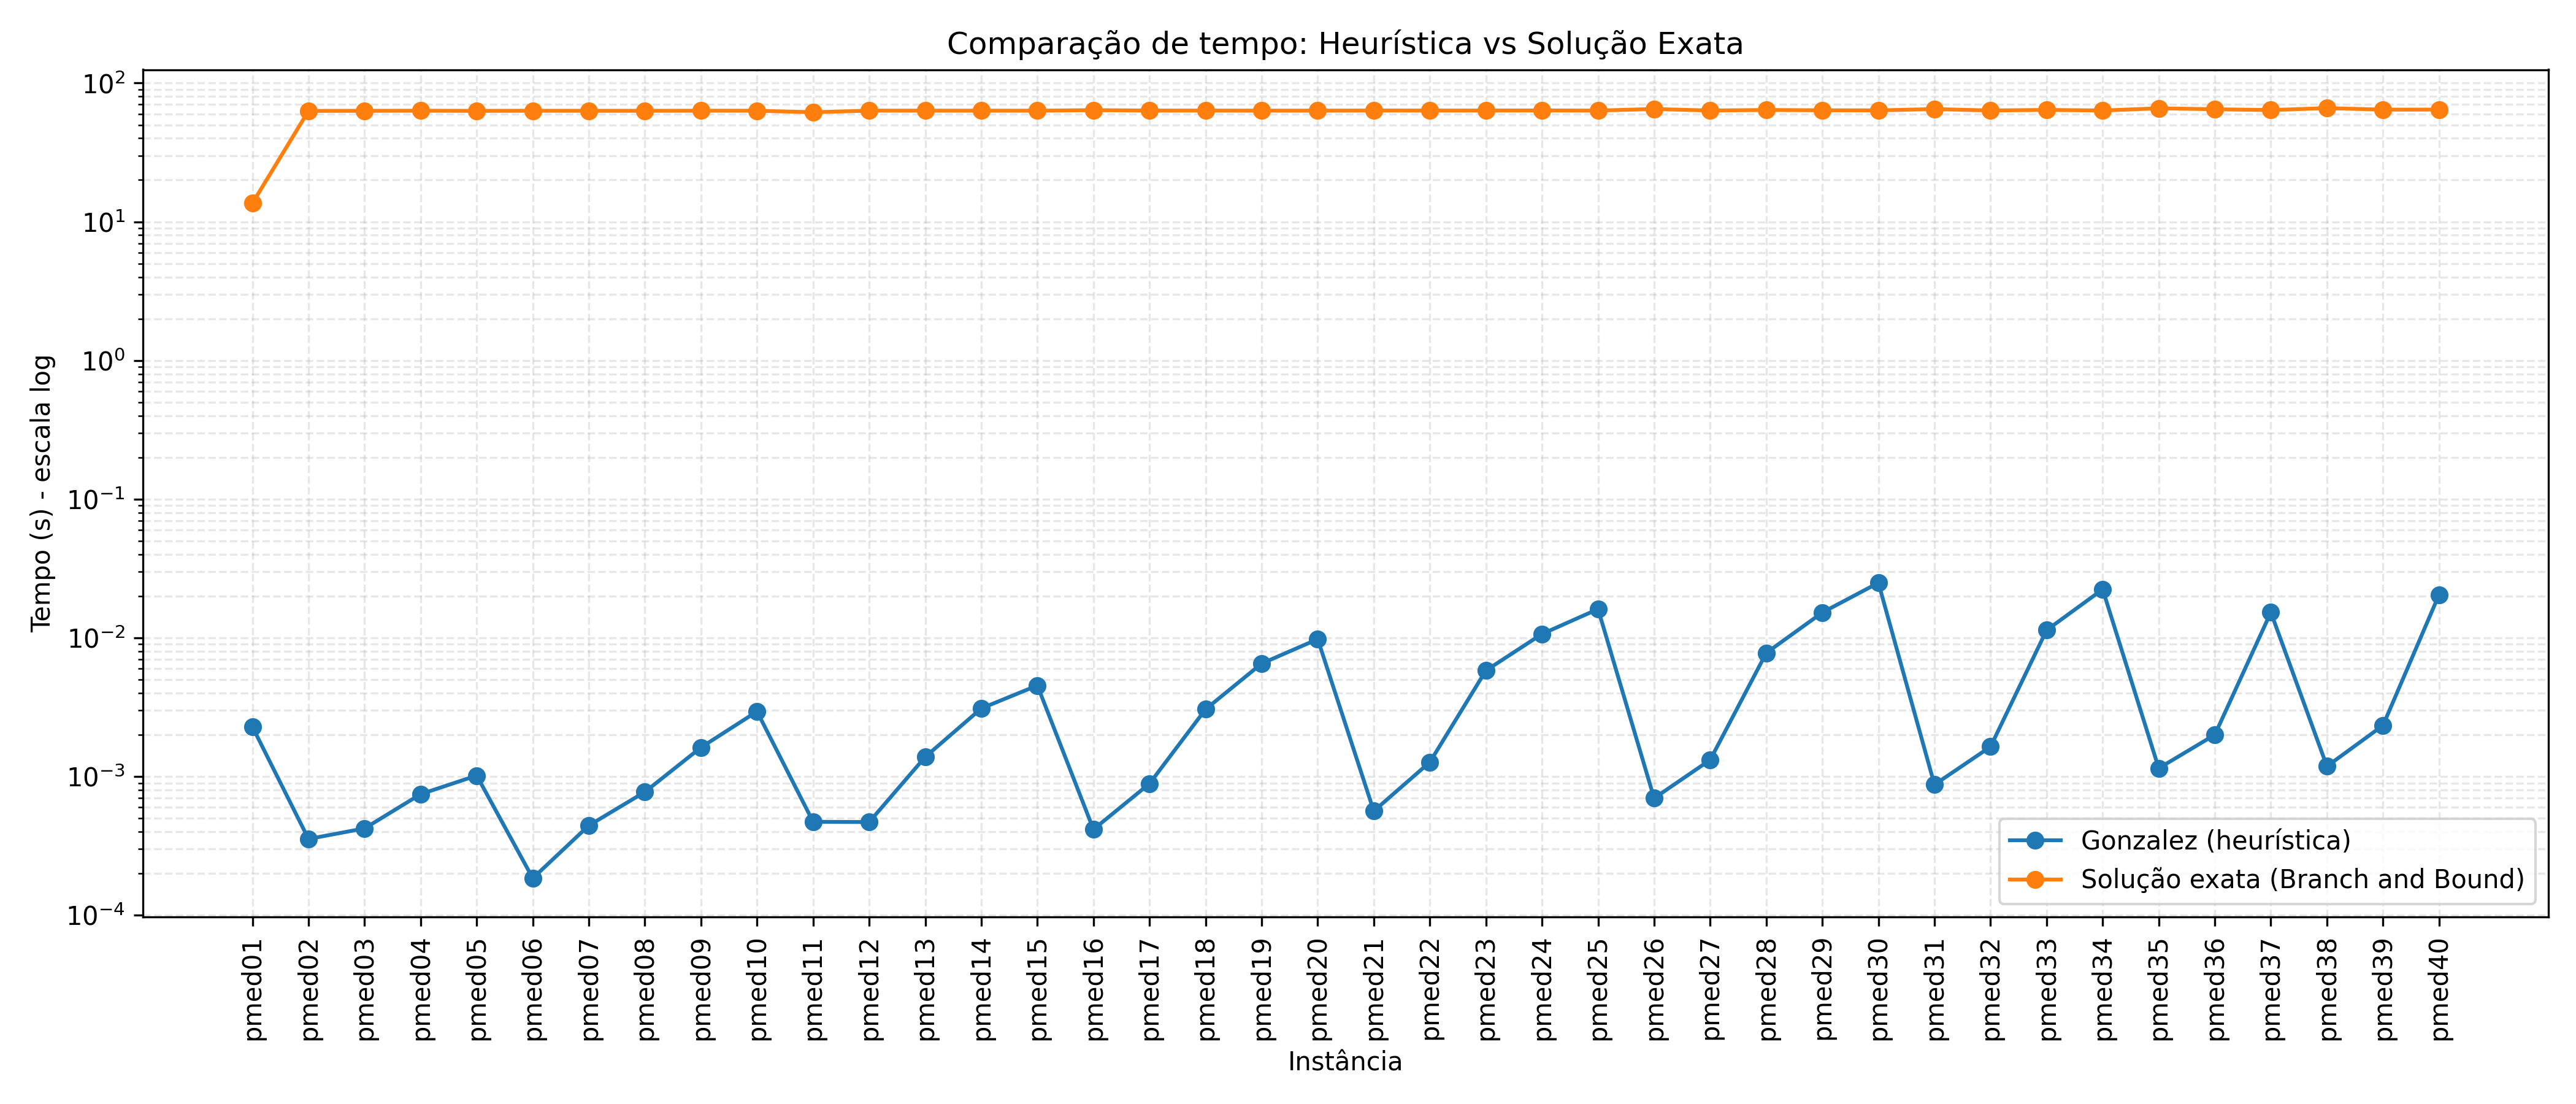
\includegraphics[width=\textwidth]{comparacao_tempo.png}
\caption{Comparação do tempo de execução entre a heurística de Gonzalez e a solução exata (Branch and Bound) para as 40 instâncias da OR-Library. A escala logarítmica foi utilizada para permitir a visualização simultânea das ordens de grandeza distintas entre os métodos.}
\label{fig:tempo-comparacao}
\end{figure}

A Figura~\ref{fig:tempo-comparacao} evidencia a grande diferença de escalabilidade entre os métodos. Enquanto a heurística de Gonzalez apresenta tempo de execução praticamente constante e na ordem de milissegundos, a solução exata permanece próxima do limite de 60 segundos para quase todas as instâncias. 

Essa diferença de ordens de grandeza reforça o impacto da explosão combinatória no método exato e justifica o uso de heurísticas para instâncias de maior porte.

\section{Análise dos Resultados}

Os resultados obtidos demonstram que a heurística de Gonzalez apresenta desempenho prático significativamente melhor do que o limite teórico garantido pela análise de aproximação. Embora a teoria assegure apenas uma solução de fator 2, as razões observadas permaneceram entre aproximadamente 1,24 e 1,79, com média próxima de 1,50.

Esse comportamento pode ser explicado pela estratégia gulosa utilizada pela heurística. Ao selecionar iterativamente o vértice mais distante dos centros já escolhidos, o algoritmo tende a distribuir os centros de forma eficiente pelo espaço da instância, reduzindo o raio máximo necessário para cobrir todos os vértices. Em muitas situações práticas, essa estratégia aproxima-se bastante da configuração ótima.

Os experimentos também mostram que o limite teórico de aproximação é conservador. Como ocorre frequentemente em algoritmos de aproximação, a análise teórica considera cenários extremos construídos especificamente para maximizar o erro do algoritmo. As instâncias da OR-Library não apresentam essas características adversas, permitindo que a heurística obtenha desempenho substancialmente melhor.

Em contraste, a solução exata sofreu fortemente com a explosão combinatória inerente ao problema. O algoritmo Branch and Bound precisa explorar um grande número de combinações possíveis de centros, e o crescimento do espaço de busca torna-se rapidamente proibitivo à medida que o número de vértices aumenta. Mesmo com mecanismos de poda, a quantidade de nós processados permaneceu elevada em praticamente todas as instâncias.

O impacto do limite de tempo também foi significativo. Embora o algoritmo exato frequentemente encontrasse soluções razoáveis antes do timeout, a incapacidade de concluir a busca impediu a comprovação da otimalidade. Consequentemente, para instâncias médias e grandes, o método deixou de fornecer uma solução garantidamente ótima dentro do orçamento computacional disponível.

De forma geral, os resultados indicam que a heurística de Gonzalez constitui uma alternativa bastante eficaz para o problema dos $k$-centros, oferecendo soluções de boa qualidade com custo computacional muito inferior ao da abordagem exata. Para instâncias de maior porte, a diferença de escalabilidade observada torna a heurística claramente mais adequada do ponto de vista prático.

\section{Como Reproduzir os Experimentos}

Todos os experimentos foram executados utilizando a implementação desenvolvida em Java e as quarenta instâncias da OR-Library disponibilizadas para o problema das p-medianas.

\subsection{Compilação}

A compilação pode ser realizada a partir do diretório raiz do projeto por meio do comando:

\begin{verbatim}
javac -d out src/*.java
\end{verbatim}

Os arquivos compilados serão armazenados no diretório \texttt{out}.

\subsection{Execução dos Testes}

Os testes automatizados utilizados para validação da implementação podem ser executados através do comando:

\begin{verbatim}
java -cp out Testes
\end{verbatim}

Ao final da execução, todos os testes devem ser aprovados.

\subsection{Experimentos com a Heurística de Gonzalez}

A execução da heurística aproximada sobre as quarenta instâncias da OR-Library é realizada pelo comando:

\begin{verbatim}
java -cp out Principal aprox
\end{verbatim}

Ao término da execução é gerado o arquivo

\begin{verbatim}
resultados_aproximado.csv
\end{verbatim}

contendo, para cada instância, o tamanho do grafo, o valor de $k$, o raio obtido pela heurística, o raio ótimo de referência, a razão entre ambos e o tempo de execução.

\subsection{Experimentos com a Solução Exata}

A solução exata pode ser executada individualmente para uma instância específica utilizando:

\begin{verbatim}
java -cp out Principal exata <instancia> [timeout]
\end{verbatim}

Por exemplo:

\begin{verbatim}
java -cp out Principal exata 1 60
\end{verbatim}

executa a instância \texttt{pmed01} com limite de tempo de 60 segundos.

Para reproduzir os experimentos realizados neste trabalho sobre todas as instâncias, utiliza-se:

\begin{verbatim}
java -cp out Principal exata_todas [timeout]
\end{verbatim}

Por exemplo:

\begin{verbatim}
java -cp out Principal exata_todas 60
\end{verbatim}

executa as quarenta instâncias utilizando limite de 60 segundos para cada uma delas.

Ao final da execução é gerado o arquivo

\begin{verbatim}
resultados_exata.csv
\end{verbatim}

contendo, para cada instância, o raio obtido, o valor ótimo de referência, o tempo de execução, o número de nós explorados pela busca e uma indicação de término normal ou interrupção por limite de tempo.

\subsection{Interface Interativa}

Opcionalmente, os experimentos também podem ser executados através da interface de linha de comando disponibilizada pela classe \texttt{Main}:

\begin{verbatim}
java -cp out Main
\end{verbatim}

A interface apresenta um menu com opções para executar a heurística, a solução exata, os testes automatizados e a geração dos arquivos CSV utilizados na análise experimental.

\section{Conclusão}

Neste trabalho foram implementadas e avaliadas duas abordagens para o problema dos $k$-centros: uma heurística aproximada baseada no algoritmo de Gonzalez e uma solução exata baseada em Branch and Bound. Ambas foram testadas utilizando as quarenta instâncias da OR-Library tradicionalmente empregadas em estudos sobre localização de facilidades.

Os resultados experimentais mostraram que a heurística de Gonzalez apresentou excelente desempenho prático. Em todas as instâncias avaliadas, as soluções encontradas respeitaram a garantia teórica de aproximação por fator 2, obtendo razões entre aproximadamente 1,24 e 1,79 em relação ao valor ótimo conhecido. Além disso, os tempos de execução permaneceram na ordem de milissegundos mesmo para as maiores instâncias, evidenciando a elevada escalabilidade do método.

Por outro lado, a abordagem exata confirmou a dificuldade computacional inerente ao problema dos $k$-centros. Embora tenha sido capaz de encontrar a solução ótima para a menor instância considerada, o crescimento combinatório do espaço de busca tornou inviável a comprovação da otimalidade para a maioria dos casos dentro do limite de tempo estabelecido. Ainda assim, os resultados obtidos permitiram observar o comportamento do método e ilustrar as limitações práticas de técnicas exatas aplicadas a instâncias de maior porte.

A comparação entre os dois métodos evidencia o tradicional compromisso entre qualidade da solução e eficiência computacional. Enquanto a abordagem exata oferece a possibilidade de encontrar a solução ótima, seu custo computacional cresce rapidamente com o tamanho da instância. Em contraste, a heurística produz soluções de boa qualidade em tempos extremamente reduzidos, tornando-se uma alternativa mais adequada para aplicações práticas envolvendo conjuntos de dados maiores.

Como trabalhos futuros, podem ser investigadas técnicas mais sofisticadas para a solução exata, incluindo estratégias adicionais de poda, formulações baseadas em programação inteira e algoritmos de busca binária sobre o valor do raio. Da mesma forma, podem ser exploradas metaheurísticas e métodos híbridos capazes de produzir soluções ainda mais próximas do ótimo sem comprometer significativamente o tempo de execução.

Em síntese, os experimentos realizados demonstraram que a heurística de Gonzalez constitui uma solução eficiente e robusta para o problema dos $k$-centros, apresentando excelente relação entre qualidade das soluções obtidas e custo computacional, especialmente quando comparada à abordagem exata em instâncias de maior porte.


\bibliographystyle{sbc}
\bibliography{references}

\end{document}
